% Provenance (never printed): NSI premiere, "Representation d'un texte en machine" (ASCII, ISO-8859-1, Unicode,
% UTF-8; identifying the encoding of a file). Mojibake repair, UTF-8 by hand and the file conversion are additions.
% See sources/book2/BRIEFS.md.
\chapter{Text Encodings: From ASCII to UTF-8}\label{ch:g10:text-encodings}

The town's café sends its weekly menu to the notice board at the station, a screen run by a small computer. On
Monday the board shows \textbf{Lighthouse Café}. The menu file has not changed, the screen is not broken, and nobody
typed an \textit{Ã}. The file and the board simply disagree about what the bytes of the file mean.

A text file is a sequence of bytes, and a byte is a number from $0$ to $255$. Turning letters into numbers and back
needs a table that both sides agree on. This chapter follows these tables from the first one, which had room for the
English alphabet only, to the one used today for every script in the world, and explains, byte by byte, how
\textit{é} became \textit{é}.

\begin{recall}
A computer stores each \omterm{def:g10:text-encodings:code-point}{character} as a number, its code, taken from a code table (Book 1, grade 5). In Python a
string is a sequence of \omterm{def:g10:text-encodings:code-point}{characters}, \code{ord(c)} gives the code of a \omterm{def:g10:text-encodings:code-point}{character} and \code{chr(n)} the \omterm{def:g10:text-encodings:code-point}{character} of a
code (Book 1, grade 7). A byte is written with two hexadecimal digits, from \code{00} to \code{FF} (Book 1,
grade 8).
\end{recall}

\section{Characters, code points and bytes}\label{sec:g10:text-encodings:code-points}

Two questions must be kept apart: which number stands for a \omterm{def:g10:text-encodings:code-point}{character}, and which bytes stand for that number.

\begin{definition}[Character, code point]\label{def:g10:text-encodings:code-point}
A \emph{character}\index{character} is a unit of written text: a letter, a digit, a punctuation sign, a space, an
emoji. A \emph{code point}\index{code point} is the number that a code table gives to a character. Code points are
written \code{U+} followed by at least four hexadecimal digits: \code{U+0041} is \textit{A}, \code{U+00E9} is
\textit{é}.
\end{definition}

\begin{definition}[Character encoding]\label{def:g10:text-encodings:encoding}
A \emph{character encoding}\index{character encoding} is a rule that turns a sequence of \omterm{def:g10:text-encodings:code-point}{characters} into a sequence of
bytes (\emph{encoding}) and back (\emph{decoding}). A text file holds bytes only; reading it as text needs the
encoding it was written with.
\end{definition}

Python keeps the two worlds apart: a \code{str} holds \omterm{def:g10:text-encodings:code-point}{characters}, a \code{bytes} value holds bytes, and the methods
\code{encode} and \code{decode} cross between them, always with the name of an \omterm{def:g10:text-encodings:encoding}{encoding}.

\section{ASCII on seven bits}\label{sec:g10:text-encodings:ascii}

\begin{definition}[ASCII]\label{def:g10:text-encodings:ascii}
% ledger: g10:ascii-1968, g10:ascii-7bit
\emph{ASCII}\index{ASCII} (American Standard Code for Information Interchange, 1968) is a code table of $128$
\omterm{def:g10:text-encodings:code-point}{characters}, numbered from $0$ to $127$, so that each fits in $7$ bits. Codes $0$ to $31$ and $127$ are
\emph{control \omterm{def:g10:text-encodings:code-point}{characters}} (line feed, tabulation, \dots), which are not printed; codes $32$ to $126$ are the space,
the digits, the English letters in both cases and punctuation. As an \omterm{def:g10:text-encodings:encoding}{encoding}, ASCII stores each \omterm{def:g10:text-encodings:code-point}{character} in one
byte whose leftmost bit is $0$.
\end{definition}

\begin{omfigure}
\begin{tikzpicture}[x=6.4mm, y=-6.4mm, font=\footnotesize]
  \fill[black!10] (0,0) rectangle (16,2);
  \fill[black!10] (15,7) rectangle (16,8);
  \fill[omDef!10] (0,3) rectangle (10,3+1) ;
  \fill[omProp!14] (1,4) rectangle (16,5) (0,5) rectangle (11,6);
  \fill[omMeth!14] (1,6) rectangle (16,7) (0,7) rectangle (11,8);
  \draw[black!40, step=1] (0,2) grid (16,8);
  \draw[black!40] (0,0) rectangle (16,2);
  \foreach \h [count=\c from 0] in {0,1,2,3,4,5,6,7,8,9,A,B,C,D,E,F}
    \node[font=\scriptsize\ttfamily, text=black!60] at (\c+0.5,-0.5) {\h};
  \foreach \r in {0,...,7} \node[font=\scriptsize\ttfamily, text=black!60, anchor=east] at (-0.1,\r+0.5) {\r x};
  \foreach \r in {2,...,7} \foreach \c in {0,...,15} {
    \pgfmathtruncatemacro{\code}{16*\r+\c}
    \ifnum\code>32 \ifnum\code<127
      \node[font=\small\ttfamily] at (\c+0.5,\r+0.5) {\ifnum\code=39 \textquotesingle\else\ifnum\code=96
        \textasciigrave\else\ifnum\code=95 \textunderscore\else\ifnum\code=126 \textasciitilde\else
        \symbol{\code}\fi\fi\fi\fi};
    \fi\fi
  }
  \node[font=\scriptsize] at (0.5,2.5) {SP};
  \node[font=\scriptsize] at (15.5,7.5) {DEL};
  \node[font=\footnotesize] at (8,1) {control characters (not printed)};
\end{tikzpicture}

{\small The \omterm{def:g10:text-encodings:ascii}{ASCII} table in rows of $16$: the row gives the first hexadecimal digit, the column the second. Digits
(blue) start at \code{30}, capital letters (orange) at \code{41} and small letters (green) at \code{61}, exactly
\code{20} hexadecimal, that is $32$, further on.}
\end{omfigure}

The layout was designed with care: the digit $d$ has code $48 + d$, and a small letter's code is the capital's plus
$32$, a single bit.

\omcode{code/grade-10/05-text-encodings/listings/ord_chr.py}{1}{4}{Codes in decimal, hexadecimal and on $7$
bits.}\label{lst:g10:text-encodings:ord-chr}

\omoutput{code/grade-10/05-text-encodings/outputs/ord_chr.txt}{\textit{A} and \textit{a} differ only in the bit
worth $32$.}\label{out:g10:text-encodings:ord-chr}

\omcode{code/grade-10/05-text-encodings/listings/ascii_table.py}{1}{7}{Printing the table of printable
\omterm{def:g10:text-encodings:code-point}{characters}.}\label{lst:g10:text-encodings:ascii-table}

\omoutput{code/grade-10/05-text-encodings/outputs/ascii_table.txt}{Rows \code{2x} to \code{7x}; the dot stands for
code $127$, which is not printable.}\label{out:g10:text-encodings:ascii-table}

\omterm{def:g10:text-encodings:ascii}{ASCII} has no \textit{é}, no \textit{ñ}, no \textit{ß}, and none of the world's other scripts. It was enough for the
teleprinters of the 1960s, which wrote English, and too little for nearly everyone else.

\begin{omfigure}
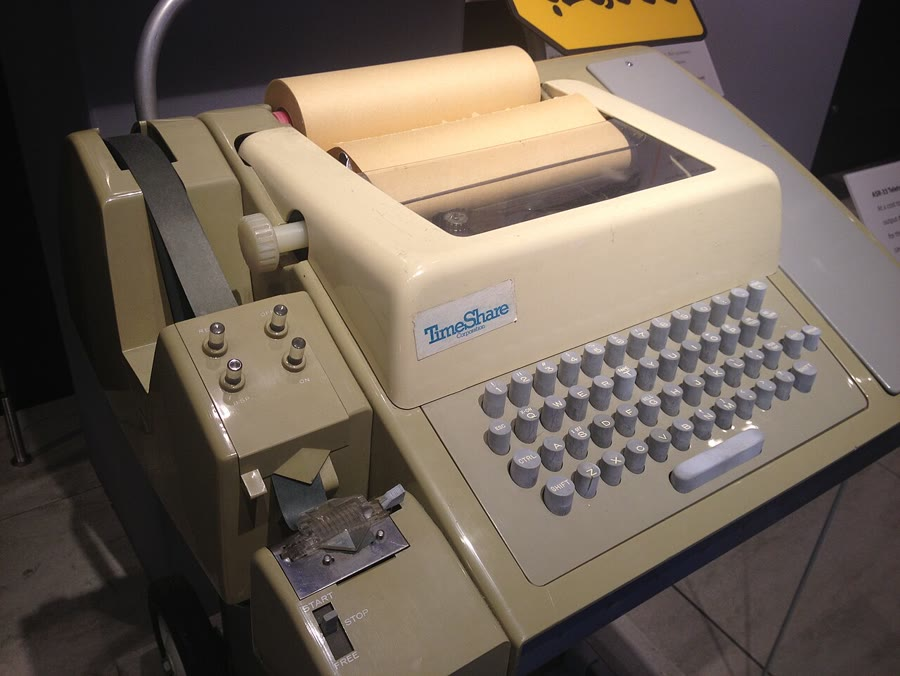
\includegraphics[width=0.5\linewidth]{images/book2/g10-teleprinter-asr33.jpg}

{\small A Teletype ASR-33 teleprinter at the Computer History Museum: a keyboard below, and a printer on a roll of
paper above. Photograph: Arnold Reinhold, CC BY-SA 3.0.}
\end{omfigure}

\section{One-byte extensions and their conflicts}\label{sec:g10:text-encodings:one-byte}

A byte has $8$ bits, and \omterm{def:g10:text-encodings:ascii}{ASCII} uses only codes $0$ to $127$. The obvious idea was to give the other $128$ values,
from $128$ to $255$, to the letters that \omterm{def:g10:text-encodings:ascii}{ASCII} lacks.

\begin{definition}[One-byte extension of ASCII]\label{def:g10:text-encodings:extension}
A \emph{one-byte extension of ASCII}\index{one-byte extension of ASCII} is an \omterm{def:g10:text-encodings:encoding}{encoding} that keeps \omterm{def:g10:text-encodings:ascii}{ASCII} for bytes $0$
to $127$ and gives bytes $128$ to $255$ to other \omterm{def:g10:text-encodings:code-point}{characters}, one \omterm{def:g10:text-encodings:code-point}{character} per byte.
% ledger: g10:latin1-1987
The best known is \emph{ISO-8859-1}\index{ISO-8859-1}, also called Latin-1 (1987), for Western European languages:
in it, byte \code{E9} is \textit{é}.
\end{definition}

The trouble is that there were dozens of such tables, one for Greek, one for Cyrillic, one for each make of computer,
and each gave the same byte a different meaning. A file does not say which table it was written with.

\omcode{code/grade-10/05-text-encodings/listings/latin1_vs_utf8.py}{1}{7}{One word, three \omterm{def:g10:text-encodings:encoding}{encodings}; one byte, two
tables.}\label{lst:g10:text-encodings:latin1-vs-utf8}

\omoutput{code/grade-10/05-text-encodings/outputs/latin1_vs_utf8.txt}{Byte \code{E9} is \textit{é} in Latin-1 and
\textit{È}, \omterm{def:g10:text-encodings:code-point}{code point} \code{U+00C8}, in an old table of another make of computer, \code{mac_roman}. The function
\code{ascii} writes a \omterm{def:g10:text-encodings:code-point}{character} that is not \omterm{def:g10:text-encodings:ascii}{ASCII} as an escape \texttt{\textbackslash x..}.}\label{out:g10:text-encodings:latin1-vs-utf8}

\begin{omfigure}
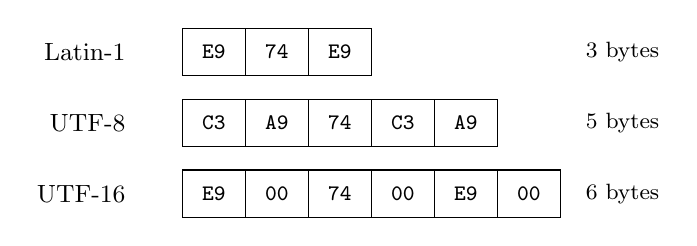
\begin{tikzpicture}[font=\small, b/.style={draw, minimum width=8mm, minimum height=6mm, font=\footnotesize\ttfamily,
    inner sep=0pt}]
  \foreach \enc/\y/\bytes/\cols in {Latin-1/0/{E9,74,E9}/{omProp!20,white,omProp!20},
      UTF-8/-0.9/{C3,A9,74,C3,A9}/{omProp!20,omProp!20,white,omProp!20,omProp!20},
      UTF-16/-1.8/{E9,00,74,00,E9,00}/{omProp!20,omProp!20,white,white,omProp!20,omProp!20}} {
    \node[anchor=east] at (-0.2,\y) {\enc};
    \foreach \bb [count=\i] in \bytes {
      \pgfmathsetmacro{\xx}{0.8*\i}
      \node[b] at (\xx,\y) {\bb};
    }
  }
  \node[anchor=west, font=\footnotesize] at (5.4,0) {3 bytes};
  \node[anchor=west, font=\footnotesize] at (5.4,-0.9) {5 bytes};
  \node[anchor=west, font=\footnotesize] at (5.4,-1.8) {6 bytes};
\end{tikzpicture}

{\small The word \textit{été} in three \omterm{def:g10:text-encodings:encoding}{encodings}. The shaded bytes stand for \textit{é}; \textit{t} is one byte in
the first two and two bytes in UTF-16, which uses at least two bytes for every \omterm{def:g10:text-encodings:code-point}{character}.}
\end{omfigure}

\section{Unicode and UTF-8}\label{sec:g10:text-encodings:unicode}

The way out was to stop making tables and make one.

\begin{definition}[Unicode]\label{def:g10:text-encodings:unicode}
% ledger: g10:unicode-1991, g10:utf8-rfc3629
\emph{Unicode}\index{Unicode} is a single code table for the \omterm{def:g10:text-encodings:code-point}{characters} of every writing system, first published in
1991. Its \omterm{def:g10:text-encodings:code-point}{code points} run from \code{U+0000} to \code{U+10FFFF}; the first $128$ are those of \omterm{def:g10:text-encodings:ascii}{ASCII} and the first
$256$ those of Latin-1. Unicode says which number each \omterm{def:g10:text-encodings:code-point}{character} has, not which bytes store it: that is the job of
an \omterm{def:g10:text-encodings:encoding}{encoding} of Unicode.
\end{definition}

\begin{dated}{2026}
% ledger: g10:unicode-18
\omterm{def:g10:text-encodings:unicode}{Unicode} 18.0, released in September 2026, contains $172{,}808$ \omterm{def:g10:text-encodings:code-point}{characters}. A new version comes out about once a
year, mostly adding \omterm{def:g10:text-encodings:code-point}{characters} of historic scripts and new emoji.
\end{dated}

Storing every \omterm{def:g10:text-encodings:code-point}{code point} in $4$ bytes would work but would make every English text four times larger. The \omterm{def:g10:text-encodings:encoding}{encoding}
used by most of the web and by almost every text file today uses between one and four bytes.

\begin{definition}[UTF-8]\label{def:g10:text-encodings:utf8}
\emph{UTF-8}\index{UTF-8} encodes each \omterm{def:g10:text-encodings:code-point}{code point} in $1$ to $4$ bytes. Its bits are placed in the free positions
\code{x} of the patterns of the figure below, from left to right. The first byte tells how many bytes follow; every
following byte, a \emph{continuation byte}, starts with the bits \code{10}.
\end{definition}

\begin{omfigure}
\begin{tikzpicture}[font=\footnotesize, every node/.style={font=\footnotesize}]
  \foreach \range/\pat/\y in {{U+0000 to U+007F}/{\textbf{0}xxxxxxx}/0,
      {U+0080 to U+07FF}/{\textbf{110}xxxxx \ \textbf{10}xxxxxx}/-0.6,
      {U+0800 to U+FFFF}/{\textbf{1110}xxxx \ \textbf{10}xxxxxx \ \textbf{10}xxxxxx}/-1.2,
      {U+10000 to U+10FFFF}/{\textbf{11110}xxx \ \textbf{10}xxxxxx \ \textbf{10}xxxxxx \ \textbf{10}xxxxxx}/-1.8} {
    \node[anchor=east] at (3.2,\y) {\range};
    \node[anchor=west, font=\footnotesize\ttfamily] at (3.5,\y) {\pat};
  }
  \node[anchor=west, font=\footnotesize, align=left] at (3.5,-2.6)
    {\textit{é} = \code{U+00E9} = \code{000 1110 1001} \ $\to$ \ \texttt{110\textcolor{omProp}{00011}} \
    \texttt{10\textcolor{omProp}{101001}} = \code{C3 A9}};
\end{tikzpicture}

{\small The four patterns of \omterm{def:g10:text-encodings:utf8}{UTF-8}, and \textit{é} encoded by hand: its $11$ bits fill the \code{x} of the two-byte
pattern.}
\end{omfigure}

% ledger: g10:utf8-surrogates
(The \omterm{def:g10:text-encodings:code-point}{code points} \code{U+D800} to \code{U+DFFF} are left out: they are reserved for UTF-16, which writes the \omterm{def:g10:text-encodings:code-point}{code
points} above \code{U+FFFF} as a pair of such numbers.)

The listing builds the bytes with the shifts and \omterm{def:g10:machine-integers:mask}{masks} of the chapter on machine integers, and checks them against
Python's own encoder.

\omcode{code/grade-10/05-text-encodings/listings/utf8_by_hand.py}{1}{19}{\omterm{def:g10:text-encodings:utf8}{UTF-8} by hand.}%
\label{lst:g10:text-encodings:utf8-by-hand}

\omoutput{code/grade-10/05-text-encodings/outputs/utf8_by_hand.txt}{\textit{A}, \textit{é}, the euro sign and an
emoji (a smiling face): $1$, $2$, $3$ and $4$ bytes.}\label{out:g10:text-encodings:utf8-by-hand}

\begin{proposition}[Properties of UTF-8]\label{prop:g10:text-encodings:utf8-properties}
\begin{enumerate}
  \item An \omterm{def:g10:text-encodings:ascii}{ASCII} text is its own \omterm{def:g10:text-encodings:utf8}{UTF-8} \omterm{def:g10:text-encodings:encoding}{encoding}, byte for byte.
  \item No byte of a \omterm{def:g10:text-encodings:code-point}{character} of two or more bytes is below $128$, so an \omterm{def:g10:text-encodings:ascii}{ASCII} byte in \omterm{def:g10:text-encodings:utf8}{UTF-8} is always an \omterm{def:g10:text-encodings:ascii}{ASCII}
    \omterm{def:g10:text-encodings:code-point}{character}.
  \item A continuation byte is never the first byte of a \omterm{def:g10:text-encodings:code-point}{character}, so a program that starts reading in the middle
    of a text finds the next \omterm{def:g10:text-encodings:code-point}{character} boundary by skipping at most three bytes.
\end{enumerate}
\end{proposition}

\begin{proof}
(1) \omterm{def:g10:text-encodings:code-point}{Code points} below $128$ use the one-byte pattern \code{0xxxxxxx}, which is the \omterm{def:g10:text-encodings:ascii}{ASCII} byte itself. (2) In a
pattern of two or more bytes, every byte starts with a $1$ bit, so it is at least $128$. (3) A continuation byte
starts with \code{10}; a first byte starts with \code{0}, \code{110}, \code{1110} or \code{11110}, never \code{10}. A
\omterm{def:g10:text-encodings:code-point}{character} has at most three continuation bytes.
\end{proof}

\section{Garbled text, and bytes in Python}\label{sec:g10:text-encodings:mojibake}

Now the notice board can be explained.

\begin{definition}[Mojibake]\label{def:g10:text-encodings:mojibake}
\emph{Mojibake}\index{mojibake (garbled text)} (garbled text, from a Japanese word) is the text obtained when bytes
are decoded with an \omterm{def:g10:text-encodings:encoding}{encoding} other than the one they were written with.
\end{definition}

\omcode{code/grade-10/05-text-encodings/listings/mojibake.py}{1}{6}{The café's name, written in \omterm{def:g10:text-encodings:utf8}{UTF-8} and read as
Latin-1.}\label{lst:g10:text-encodings:mojibake}

\omoutput{code/grade-10/05-text-encodings/outputs/mojibake.txt}{The wrong reading has one \omterm{def:g10:text-encodings:code-point}{character} more than the
name: the two bytes of \textit{é} became two \omterm{def:g10:text-encodings:code-point}{characters}, \texttt{\textbackslash xc3} and \texttt{\textbackslash xa9}. \omterm{def:g10:text-encodings:encoding}{Encoding} back and decoding
right repairs it.}\label{out:g10:text-encodings:mojibake}

\begin{omfigure}
\begin{tikzpicture}[font=\small, node distance=18mm, s/.style={draw, rounded corners=2pt, minimum height=8mm,
    inner sep=4pt}]
  \node[s, fill=omDef!8] (a) {\textit{é}};
  \node[s, right=of a, font=\small\ttfamily] (b) {C3 A9};
  \node[s, right=of b, fill=omProp!14] (c) {\textit{Ã} \quad \textit{©}};
  \draw[ptr] (a) -- node[above, font=\footnotesize] {UTF-8} (b);
  \draw[ptr] (b) -- node[above, font=\footnotesize] {Latin-1} (c);
  \node[below=1mm of a, font=\footnotesize] {\code{U+00E9}};
  \node[below=1mm of b, font=\footnotesize] {two bytes};
  \node[below=1mm of c, font=\footnotesize] {\code{U+00C3}, \code{U+00A9}};
\end{tikzpicture}

{\small The path from \textit{é} to \textit{é}: written with one \omterm{def:g10:text-encodings:encoding}{encoding}, read with another. In Latin-1, byte
\code{C3} is \textit{Ã} and byte \code{A9} is the copyright sign \textit{©}.}
\end{omfigure}

\begin{method}[Recognising the encoding of garbled text]\label{met:g10:text-encodings:recognise}
\begin{enumerate}
  \item An accented letter replaced by two \omterm{def:g10:text-encodings:code-point}{characters}, the first often \textit{Ã} or \textit{Â}: \omterm{def:g10:text-encodings:utf8}{UTF-8} bytes read as
    Latin-1 (or as a close one-byte table). Repair: encode with Latin-1, decode with \omterm{def:g10:text-encodings:utf8}{UTF-8}.
  \item A replacement sign, or the error \code{UnicodeDecodeError}: one-byte-table bytes read as \omterm{def:g10:text-encodings:utf8}{UTF-8}. Decode with the
    right one-byte table.
  \item Three or four \omterm{def:g10:text-encodings:code-point}{characters} for one letter: the mistake was made twice; repair once per layer.
\end{enumerate}
\end{method}

Decoding does not always succeed. Byte \code{E9} starts a three-byte \omterm{def:g10:text-encodings:code-point}{character} in \omterm{def:g10:text-encodings:utf8}{UTF-8}, so a Latin-1 \textit{é} at
the end of a text is an incomplete \omterm{def:g10:text-encodings:utf8}{UTF-8} \omterm{def:g10:text-encodings:code-point}{character}.

\omcode{code/grade-10/05-text-encodings/listings/decode_error.py}{2}{5}{Latin-1 bytes read as
\omterm{def:g10:text-encodings:utf8}{UTF-8}.}\label{lst:g10:text-encodings:decode-error}

\omoutput{code/grade-10/05-text-encodings/outputs/decode_error.txt}{\code{errors="backslashreplace"} writes
the bad byte as an escape; without it, decoding stops.}\label{out:g10:text-encodings:decode-error}

With \code{errors="replace"}, Python puts the replacement \omterm{def:g10:text-encodings:code-point}{character} \code{U+FFFD}, usually drawn as a question mark
in a diamond, in place of each bad byte; with the default, \code{errors="strict"}, it stops.

\begin{method}[Reading and writing text files]\label{met:g10:text-encodings:files}
Always name the \omterm{def:g10:text-encodings:encoding}{encoding}: \code{open(name, encoding="utf-8")}, \code{Path(name).read_text(encoding="utf-8")}. Without
it, Python uses the system's default, which is not the same on every computer. To convert a file, read it with its
old \omterm{def:g10:text-encodings:encoding}{encoding} and write it with the new one.
\end{method}

\omcode{code/grade-10/05-text-encodings/listings/convert_file.py}{2}{13}{Converting a menu from a one-byte table to
\omterm{def:g10:text-encodings:utf8}{UTF-8}.}\label{lst:g10:text-encodings:convert-file}

\omoutput{code/grade-10/05-text-encodings/outputs/convert_file.txt}{\textit{é}, \textit{ê} and the euro sign take one
byte each in the old file and $2$, $2$ and $3$ bytes in \omterm{def:g10:text-encodings:utf8}{UTF-8}: $4$ bytes more.}\label{out:g10:text-encodings:convert-file}

The table used here, \code{cp1252}, is a one-byte table close to Latin-1 that has the euro sign at byte \code{80}.

\section{Exercises}\label{sec:g10:text-encodings:exercises}

\begin{exercise}[$\star$]\label{exo:g10:text-encodings:1}
What do \code{ord("A")}, \code{chr(97)}, \code{ord("9") - ord("0")} and \code{chr(ord("A") + 2)} return?
\end{exercise}

\begin{exercise}[$\star$]\label{exo:g10:text-encodings:2}
Give the bytes, in hexadecimal, of the word \textit{été} in Latin-1 and in \omterm{def:g10:text-encodings:utf8}{UTF-8}, using the figure of \omterm{def:g10:text-encodings:utf8}{UTF-8} patterns,
and check them against the listing.
\end{exercise}

\begin{exercise}[$\star$]\label{exo:g10:text-encodings:3}
What do \code{len("Café")}, \code{len("Café".encode("utf-8"))} and \code{len("Café".encode("latin-1"))} return?
Explain the difference.
\end{exercise}

\begin{exercise}[$\star$]\label{exo:g10:text-encodings:4}
Write the codes of \textit{A} and \textit{a} on $7$ bits and show that they differ by one bit. Deduce a way to change
the case of an \omterm{def:g10:text-encodings:ascii}{ASCII} letter with one \omterm{def:g10:machine-integers:bitwise}{bitwise operation}.
\end{exercise}

\begin{exercise}[$\star$]\label{exo:g10:text-encodings:5}
Write \code{is_ascii(s)}, which tells whether every \omterm{def:g10:text-encodings:code-point}{character} of the string \code{s} is an \omterm{def:g10:text-encodings:ascii}{ASCII} \omterm{def:g10:text-encodings:code-point}{character}, using
\code{ord}.
\end{exercise}

\begin{exercise}[$\star\star$]\label{exo:g10:text-encodings:6}
Decode by hand the \omterm{def:g10:text-encodings:utf8}{UTF-8} bytes \code{63 72 C3 AA 70 65}: split them into \omterm{def:g10:text-encodings:code-point}{characters} with the first bytes, then
compute each \omterm{def:g10:text-encodings:code-point}{code point}.
\end{exercise}

\begin{exercise}[$\star\star$]\label{exo:g10:text-encodings:7}
Write \code{utf8_length(cp)}, which returns the number of \omterm{def:g10:text-encodings:utf8}{UTF-8} bytes of a \omterm{def:g10:text-encodings:code-point}{code point}, and test it against
\code{len(chr(cp).encode())}.
\end{exercise}

\begin{exercise}[$\star\star$]\label{exo:g10:text-encodings:8}
A program reads a \omterm{def:g10:text-encodings:utf8}{UTF-8} file of town names with \code{open(name, encoding="latin-1")} and prints
\textit{Lighthouse Café}. Which item of the method on garbled text is this? Correct the program, and say how to
repair a string already read wrongly.
\end{exercise}

\begin{exercise}[$\star\star$]\label{exo:g10:text-encodings:9}
The bytes \code{43 61 66 E9 20 63 72 EA 70 65} are \textit{Café crêpe} in Latin-1. What does decoding them as
\omterm{def:g10:text-encodings:utf8}{UTF-8} with \code{errors="replace"} return? How many replacement \omterm{def:g10:text-encodings:code-point}{characters}
appear, and why does the error handler matter for a program that reads files from many sources?
\end{exercise}

\begin{exercise}[$\star\star$]\label{exo:g10:text-encodings:10}
How many \omterm{def:g10:text-encodings:code-point}{code points} can the two-byte pattern of \omterm{def:g10:text-encodings:utf8}{UTF-8} hold in its $11$ free bits? Why does \omterm{def:g10:text-encodings:utf8}{UTF-8} use it only for
\code{U+0080} to \code{U+07FF}, and how many \omterm{def:g10:text-encodings:code-point}{code points} is that?
\end{exercise}

\begin{exercise}[$\star\star$]\label{exo:g10:text-encodings:11}
To fit a 4-byte field of a form, a program keeps the first $4$ bytes of a name's \omterm{def:g10:text-encodings:utf8}{UTF-8} \omterm{def:g10:text-encodings:encoding}{encoding} and decodes them. For
\textit{Café} it stops with an error. Explain, and write \code{cut(text, n)}, which returns the longest beginning of
\code{text} whose \omterm{def:g10:text-encodings:utf8}{UTF-8} \omterm{def:g10:text-encodings:encoding}{encoding} has at most \code{n} bytes.
\end{exercise}

\begin{exercise}[$\star\star\star$]\label{exo:g10:text-encodings:12}
Write \code{utf8_decode(data)}, which returns the list of \omterm{def:g10:text-encodings:code-point}{code points} of valid \omterm{def:g10:text-encodings:utf8}{UTF-8} bytes, with the shifts and \omterm{def:g10:machine-integers:mask}{masks}
of the chapter on machine integers, and test it against Python's \code{decode} on random \omterm{def:g10:text-encodings:code-point}{code points}.
\end{exercise}

\begin{exercise}[$\star\star\star$]\label{exo:g10:text-encodings:13}
Prove that in valid \omterm{def:g10:text-encodings:utf8}{UTF-8} a sequence of bytes that is the \omterm{def:g10:text-encodings:encoding}{encoding} of a \omterm{def:g10:text-encodings:code-point}{character} never appears inside the \omterm{def:g10:text-encodings:encoding}{encoding}
of a longer \omterm{def:g10:text-encodings:code-point}{character}. Deduce that searching for the bytes of a word inside the bytes of a text never finds a false
match that starts in the middle of a \omterm{def:g10:text-encodings:code-point}{character}.
\end{exercise}

\begin{exercise}[$\star\star\star$]\label{exo:g10:text-encodings:14}
Write \code{fix_mojibake(s)}, which undoes one layer of \omterm{def:g10:text-encodings:utf8}{UTF-8} read as Latin-1 when that is possible and returns
\code{s} unchanged otherwise. Why is \code{fix_mojibake("Café")} equal to \textit{Café}?
\end{exercise}

\begin{exercise}[$\star\star\star$]\label{exo:g10:text-encodings:15}
A text has $10{,}000$ \omterm{def:g10:text-encodings:code-point}{characters}: $9{,}000$ \omterm{def:g10:text-encodings:ascii}{ASCII} \omterm{def:g10:text-encodings:code-point}{characters}, $900$ accented Latin letters and $100$ euro signs. Give
its size in bytes in \omterm{def:g10:text-encodings:utf8}{UTF-8}, in UTF-16 and in a one-byte table that has all these \omterm{def:g10:text-encodings:code-point}{characters}. When would UTF-16 be the
smaller of the first two?
\end{exercise}

\section{Problem: The Notice Board}\label{sec:g10:text-encodings:problem}

\begin{problem}[{Weekend problem --- what the station screen shows}]\label{pb:g10:text-encodings:1}
The station's notice board receives the café's message as a file of bytes. The program
\code{exercises/notice_board.py} prints the bytes of the message, garbles it once and twice, and counts the bytes of
the town's place names in three \omterm{def:g10:text-encodings:encoding}{encodings}.

\medskip\noindent\textbf{Part I --- A byte dump.}
\begin{enumerate}
  \item The file begins \code{4c 69 67 68 74 68 6f 75 73 65 20 43 61 66 c3 a9}. Using the \omterm{def:g10:text-encodings:ascii}{ASCII} table, decode the
    first $14$ bytes.
  \item Which bytes are not \omterm{def:g10:text-encodings:ascii}{ASCII}? Using the \omterm{def:g10:text-encodings:utf8}{UTF-8} patterns, decode them to one \omterm{def:g10:text-encodings:code-point}{code point} and name the \omterm{def:g10:text-encodings:code-point}{character}.
  \item The second line of the dump is \code{3a 20 63 72 c3 aa 70 65 73 20 74 6f 64 61 79}. Decode it.
  \item How many \omterm{def:g10:text-encodings:code-point}{characters} and how many bytes does the whole message have?
\end{enumerate}

\medskip\noindent\textbf{Part II --- Which encoding?}
\begin{enumerate}[resume]
  \item Could these bytes be Latin-1? What would the board show then?
  \item Could they be pure \omterm{def:g10:text-encodings:ascii}{ASCII}? Why not?
  \item Explain why a valid \omterm{def:g10:text-encodings:utf8}{UTF-8} reading is strong evidence that the file is \omterm{def:g10:text-encodings:utf8}{UTF-8}: what would a Latin-1 text have to
    contain for its bytes to be valid \omterm{def:g10:text-encodings:utf8}{UTF-8} by chance?
  \item The board shows \textit{Lighthouse Café: crêpes today}. Which \omterm{def:g10:text-encodings:encoding}{encoding} did the board use, and which item of
    the method does this match?
\end{enumerate}

\medskip\noindent\textbf{Part III --- Two layers.}
\begin{enumerate}[resume]
  \item A second, older screen copies the garbled text, saves it in \omterm{def:g10:text-encodings:utf8}{UTF-8}, and reads it back as Latin-1. Using the
    program's output, how is \textit{é} written after two layers? Give the four \omterm{def:g10:text-encodings:code-point}{code points}.
  \item How many bytes does \textit{é} take in \omterm{def:g10:text-encodings:utf8}{UTF-8} after one layer, and after two?
  \item Show that each layer at least doubles the number of bytes of every \omterm{def:g10:text-encodings:ascii}{non-ASCII} \omterm{def:g10:text-encodings:code-point}{character}.
  \item Undo the two layers in Python with the function \code{ungarble} of the program, and say in which order the
    two operations are applied at each step.
  \item What happens to the \omterm{def:g10:text-encodings:ascii}{ASCII} \omterm{def:g10:text-encodings:code-point}{characters} of the message through the layers, and why?
\end{enumerate}

\medskip\noindent\textbf{Part IV --- The town's names.}
\begin{enumerate}[resume]
  \item The town has $30$ places. How many bytes do their names take in \omterm{def:g10:text-encodings:utf8}{UTF-8}, in UTF-16 and in Latin-1, according
    to the program?
  \item Explain why the UTF-16 total is exactly twice the number of \omterm{def:g10:text-encodings:code-point}{characters}.
  \item Explain why the \omterm{def:g10:text-encodings:utf8}{UTF-8} total is one more than the Latin-1 total.
  \item How many bytes does \omterm{def:g10:text-encodings:utf8}{UTF-8} save over UTF-16 on these names, and what fraction is that?
  \item If the café were renamed with a Greek word of $6$ letters (each Greek letter has a \omterm{def:g10:text-encodings:code-point}{code point} between
    \code{U+0370} and \code{U+03FF}), how would each total change?
  \item State the result: the sizes of the town's names in the three \omterm{def:g10:text-encodings:encoding}{encodings}, the saving of \omterm{def:g10:text-encodings:utf8}{UTF-8} over UTF-16, and
    the rule that turns \textit{é} into \textit{é}.
\end{enumerate}
\end{problem}
